\documentclass[12pt]{galois-whitepaper}
\usepackage{listings}
\usepackage{float}
\usepackage{xspace}
\usepackage{color}
\usepackage{tikz}
\usepackage{url}
\usepackage{amsmath}
\usepackage{amsfonts}
\usepackage{amssymb}
\usepackage{amscd}
\usepackage{verbatim}
\usepackage{subcaption}
\usepackage{fancyvrb}
\let\verbatiminput=\verbatimtabinput
\VerbatimFootnotes
\DefineVerbatimEnvironment{code}{Verbatim}{}
\DefineVerbatimEnvironment{pseudoCode}{Verbatim}{}
%\hyphenation{Saw-Script}
%\newcommand{\sawScript}{{\sc SawScript}\xspace}

\usepackage[all,2cell]{xy}
\UseAllTwocells

\usepackage{textcomp}

\renewcommand{\textfraction}{0.05}
\renewcommand{\topfraction}{0.95}
\renewcommand{\bottomfraction}{0.95}
\renewcommand{\floatpagefraction}{0.35}
\setcounter{totalnumber}{5}
\definecolor{MyGray}{rgb}{0.9,0.9,0.9}
\makeatletter\newenvironment{graybox}{%
   \begin{lrbox}{\@tempboxa}\begin{minipage}{\columnwidth}}{\end{minipage}\end{lrbox}%
   \colorbox{MyGray}{\usebox{\@tempboxa}}
}\makeatother

\setlength{\parskip}{0.6em}
\setlength{\abovecaptionskip}{0.5em}

\lstset{
         basicstyle=\footnotesize\ttfamily, % Standardschrift
         %numbers=left,               % Ort der Zeilennummern
         numberstyle=\tiny,          % Stil der Zeilennummern
         %stepnumber=2,               % Abstand zwischen den Zeilennummern
         numbersep=5pt,              % Abstand der Nummern zum Text
         tabsize=2,                  % Groesse von Tabs
         extendedchars=true,         %
         breaklines=true,            % Zeilen werden Umgebrochen
         keywordstyle=\color{red},
                frame=lrtb,         % left, right, top, bottom frames.
 %        keywordstyle=[1]\textbf,    % Stil der Keywords
 %        keywordstyle=[2]\textbf,    %
 %        keywordstyle=[3]\textbf,    %
 %        keywordstyle=[4]\textbf,   \sqrt{\sqrt{}} %
         stringstyle=\color{white}\ttfamily, % Farbe der String
         showspaces=false,           % Leerzeichen anzeigen ?
         showtabs=false,             % Tabs anzeigen ?
         xleftmargin=10pt, % was 17
         xrightmargin=5pt,
         framexleftmargin=5pt, % was 17
         framexrightmargin=-1pt, % was 5pt
         framexbottommargin=4pt,
         %backgroundcolor=\color{lightgray},
         showstringspaces=false      % Leerzeichen in Strings anzeigen ?
}

\author{Eric Davis, Alec Theriault, and Ryan Wright}
\title{September ASKE Milestone Report for AMIDOL}
\date{9/30/2019}
\begin{document}
\maketitle

\vspace*{2cm}
\tableofcontents

\section{Milestone 8: Interim Code Release}

Recent work on AMIDOL has benefited from collaborations with our
colleagues from GTRI and the University of Arizona, leading to
expanded scope and capabilities in our tool.  We have released the
next version of AMIDOL at its github site
(\url{https://github.com/GaloisInc/AMIDOL/}) under the BSD 3-Clause
``New'' or ``Revised'' License.

AMIDOL has been expanded in several
fundamental ways, including new support for direct model comparisons.
Building towards a rich capability to compare the results of
comparable measures for multiple models, AMIDOL current supports
comparing measures from:

\begin{itemize}
\item The same model.
\item The same model run with different solvers.
\item Different models.
\item Models and real data.
\end{itemize}

We expect to continue to expand these capabilities with a full algebra
on measures to support more sophisticated comparisons and tests.

AMIDOL has also been extended to provide functionality for lifting
code and groundings, implemented in Julia, into AMIDOL's VDSOL-based
\textbf{abstract knowledge layer}.  Julia source files are first
transformed into the AMIDOL \textbf{structural knowledge layer} using
our process algebra-based IR.  These representations are then divided
into separate elements, and AMIDOL performs \textbf{palette-} and
\textbf{formulation-inference} to create a VDSOL palette, and a
formulation using that palette.  Palette elements use grounding
information included in the Julia source to try and augment VDSOL
elements with visual representations and composition rules by
searching over an annotated version of the SNOMED CT ontology.

AMIDOL has also been expanded to support a richer IR.  The updated
AMIDOL IR supports general input predicates (conditions which must be
met for an event to fire and change state, the equivalent of inhibator
arcs in Petri-nets).  AMIDOL has also extended its IR with support for
general output predicates, allowing for side-effects of an event
firing to be represented by arbitrary functions.  AMIDOL has expanded
its state-sharing mechanism to allow composition by general rules
defined by double-push-out diagrams given in applied category theory.

AMIDOL's UI has also been extended to improve the user experience, and
satisfy the needs of the new palette and formulation inference
procedures.  VDSOL palette elements now have a modification work-flow
that can be followed through the GUI.  The General UI/UX was also
updated to allow for multiple client connections at a single time,
separating the state of the client by user.  This was done to
facilitate broader demos to multiple audiences, and to better enable
us to share our results with the community.

  \section{Milestone 9: Interim Status Report}

  \subsection{Machine-Generation and Evaluation of Expert Hypothesis}

  \begin{figure}
    \centering
    \includegraphics[width=0.5\textwidth]{knowledgespider.png}
    \caption{The ASKE Modeling Stack}
    \label{Fig:Stack}
  \end{figure}
  
  One of the primary goals of the ASKE program is to remove the burden
  of working with \textbf{executable knowledge} (i.e. source code in a
  given language, or compiled for a targeted architecture) and
  \textbf{structured knowledge} (i.e. mathematics outside of a
  specific domain context) by enabling domain experts and scientists
  to interact with an \textbf{abstract knowledge} layer, as shown in
  Figure \ref{Fig:Stack}.  Current state-of-the-art methods require
  domain scientists to essentially be experts in, not only domain
  science, but also in mathematics, statistics, software engineering,
  even possibly machine learning and data science, all in addition to
  expertise in their own domain.  This is an unacceptable burden which
  creates unrealistic expectations on mastery of these core skills,
  and leads to poor implementations, bugs, errors, and long
  development times resulting in applications, simulations, and models
  with poor performance and the potential for serious errors,
  inaccuracies, and correctness problems.
  
  \begin{figure}
    \centering
    \includegraphics[width=\textwidth]{high-level-abstraction.png}
    \caption{Mapping abstractions to Visual Domain Specific Languages (VDSOLs).}
    \label{Fig:Abstraction}
  \end{figure}

  One of the primary ways AMIDOL addresses these issues is in its use
  of Visual Domain Specific Ontological Languages (VDSOLs) for
  \textbf{model and measure formulation}.  VDSOLs help achieve these
  goals by lowering the barrier for entry associated with formal
  modeling languages. VDSOLs allow the expression of rich mathematical
  concepts using visual diagrams for systems and processes, but back
  these visual diagrams with a rich mathematical language, the AMIDOL
  IR, and execution semantics.  This approach enables domain experts
  to build models of complex systems which are easier to maintain,
  validate, and verify, and avoid common pitfalls of monolithic and
  hand-coded implementations.

  Figure \ref{Fig:Abstraction} shows an example of a model in an
  example formulation palette for AMIDOL, and the mapping of its
  mathematical meaning to a system of differential equations that
  represents the same model.  AMIDOL can automatically translate the
  diagram into the provided system of equations, and solve the
  resulting system for measures defined on the formulation.
  
  \begin{figure}
    \centering
    \includegraphics[width=\textwidth]{vdsol-formulations.png}
    \caption{Example Formulations of two models in two separate languages.}
    \label{Fig:Formulations}
  \end{figure}

  The purpose of VDSOLs is not to be prescriptive or restrictive,
  limiting users to a single language or representation.  Figure
  \ref{Fig:Formulations}, for instance, shows two separate models (SIR
  and SIIR model respectively on the top and the bottom) implemented
  in two separate VDSOLs.  Those on the left using a directed
  graph-based VDSOL with noun and verb separations; and those on the
  right using a language of stochastic reactions much like
  \texttt{DiffEqBiological.jl}.  Each pair of models represents the
  same underlying system and, in fact, has the same representation in
  the AMIDOL IR.  VDSOLs allow scientists and domain experts to
  express models in a familiar syntax, and also to lift
  representations in the AMIDOL IR into a familiar syntax,
  automatically, even when they were originally authored in a
  different language.

  AMIDOL's process of formulation inference even allows new palettes
  and languages to be constructed given extant code, and annotations
  of a domain-specific ontology, such as SNOMED CT.

\subsection{Formal Rules for Composing the AMIDOL IR}

We have extended our previously provided AMIDOL IR with formal rules
for composition of \textbf{atomic models} in a VDSOL, formed of
arbitrary sets of state-variables and events in the AMIDOL IR.  This
formal set of rules allows us not only to formalize the state-sharing
process mentioned in prior reports, but also provides formal rules for
composing models in formulated palettes, and checking compositions to
ensure they are correct.

To do so, we utilize existing proofs from Applied Category Theory.  We
consider any model in the AMIDOL IR as a process algebra represented
by the morphism \[P: X \nrightarrow Y.\]  We treat this representation
as an open graph.  We build three rules for composing elements of the
AMIDOL IR providing for \textbf{parallel} and \textbf{serial
  composition}, and a rule for \textbf{substitution}.

  \paragraph{Parallel composition.}   Parallel composition of two
  models in the AMIDOL IR is accomplished by tensoring two models $P$
  and $Q$ via disjoint union, \[P \oplus Q: X_0 \oplus Y_1
    \nrightarrow Y_0 \oplus Z_1.\]  

  \begin{figure}
    \centering
    \begin{subfigure}[b]{0.45\textwidth}
      \includegraphics[width=\textwidth]{parallel-1.png}
      \caption{Two AMIDOL IR representations prior to parallel composition.}
      \label{Fig:Parallel-1}
    \end{subfigure}
        \begin{subfigure}[b]{0.45\textwidth}
      \includegraphics[width=\textwidth]{parallel-2.png}
      \caption{Two AMIDOL IR representations after parallel composition.}
      \label{Fig:Parallel-2}
    \end{subfigure}
    \caption{Example of parallel composition in the AMIDOL IR.}
    \label{Fig:Parallel}
  \end{figure}

This results, as shown in Figure \ref{Fig:Parallel} in a new symmetric
monodial category which is also a valid model in the AMIDOL IR.
  
\paragraph{Serial composition.}  Serial composition of two models in
the AMIDOL IR is accomplished by the application of the cospan from
$X$ to $Z$ resulting in $P \odot Q: X \nrightarrow Z$,

    \centerline{
    \xymatrix{
     & & P +_{Y} Q & & \\
    & P \ar[ur]^{j_P}& & \ar[ul]_{j_Q} Q & \\
    X \ar[ur]^{i_1} & & \ar[ul]_{o_1} Y \ar[ur]^{i_2} & & \ar[ul]_{o_2} Z \\
    }
  }

  \begin{figure}
    \centering
    \begin{subfigure}[b]{0.45\textwidth}
      \includegraphics[width=\textwidth]{series-1.png}
      \caption{Two AMIDOL IR representations prior to serial composition.}
      \label{Fig:Parallel-1}
    \end{subfigure}
    \begin{subfigure}[b]{0.45\textwidth}
      \centering
      \includegraphics[width=0.67\textwidth]{series-2.png}
      \caption{Two AMIDOL IR representations after serial composition.}
      \label{Fig:Parallel-2}
    \end{subfigure}
    \caption{Example of serial composition in the AMIDOL IR.}
    \label{Fig:Serial}
  \end{figure}

The results of this process are shown in Figure \ref{Fig:Serial}.
  
  \paragraph{Substitution rules.} Lastly, we provide a rule for
  substitution, this is usful for automatic model variation, as well
  as for our process of palette formulation, wherein specific models
  are generated from an annotated ontology to match ``signatures'' of
  models using AMIDOL IR models extracted from found code.
  Substitutional rules utilizes double-push-out diagrams,

    \centerline{
    \xymatrix{
    l \ar[r] \ar[d] & \ar[d] k & \ar[d] \ar[l] r\\
    g \ar[r] & d & \ar[l] h
    }
  }

Where intuitively $l$ contains the original model, $r$ contains the
substituted model, and $k$ contains the invariants in $l$ and $r$.
The model $g$ then represents a model which contains a ``copy'' of
$l$, and $h$ is equivalent to $g$ with its copy of $l$ substituted
with $r$, with $d$ describing the invariants.
  
  \begin{figure}
    \centering
    \begin{subfigure}[b]{0.3\textwidth}
      \includegraphics[width=\textwidth]{petri-net.png}
      \caption{Original model, $l$.}
      \label{Fig:Sub-L}
    \end{subfigure}
    \begin{subfigure}[b]{0.3\textwidth}
      \includegraphics[width=\textwidth]{signature.png}
      \caption{Model invariants, $k$.}
      \label{Fig:Sub-K}
    \end{subfigure}
    \begin{subfigure}[b]{0.3\textwidth}
      \includegraphics[width=\textwidth]{petri-net2.png}
      \caption{Substituted model, $r$.}
      \label{Fig:Sub-R}
    \end{subfigure}
    \begin{subfigure}[b]{0.45\textwidth}
      \includegraphics[width=\textwidth]{series-2.png}
      \caption{Model $g$, which contains a copy of $l$.}
      \label{Fig:Sub-G}
    \end{subfigure}
    \begin{subfigure}[b]{0.45\textwidth}
      \includegraphics[width=\textwidth]{substitution-1.png}
      \caption{Model $h$, where $g$'s copy of $l$ has been replaced by
        $r$.}
      \label{Fig:Sub-H}
    \end{subfigure}
    \caption{AMIDOL IR's substitution rule, illustrated.}
    \label{Fig:Substitution}
  \end{figure}

Figure \ref{Fig:Substitution} shows this process with an example
model.

\subsection{Interpretation of Model Outputs to Identify Novel
    Characteristics or Flaws}

Substitution provides us with a way to reason about the compatibility,
or incompatibility, of two models defined in the AMIDOL IR, giving us
better ability to help diagnose potential errors or problems in model
formulation, or to find possible model variations of interest using
similar proofs from Applied Category Theory.  For instance, provided
we have $P: X \nrightarrow Y$ and $Q: X \nrightarrow Y$,

\begin{center}
  \xymatrix@+2pc{
    X \rtwocell^l_r{\alpha} &Y\\
  }
\end{center}

allows us to reason about the compatibility of $P$ and $Q$, namely
 that two models in the AMIDOL IR are compatible if a substitution
 morphism $\alpha: P \nrightarrow Q$ can be constructed that follows
 our substitution rules, and maintains as invariants $X$ and $Y$.

   \begin{figure}
    \centering
    \includegraphics[width=0.5\textwidth]{AMIDOL-graph.png}
    \caption{Representing Model Comparison in the ASKE Modeling Stack
      with the Results Graph}
    \label{Fig:Results}
  \end{figure}

  We are working to further extend AMIDOL to allow for easy model
  comparison through the implementation of capabilities to perform
  algebra on the results of model execution, using a database to store
  the results of model execution and measure evaluation, represented
  in Figure \ref{Fig:Results}.

  AMIDOL's graph database will consist of a set of nodes, $M = \{M_0,
  M_1, \ldots\}$ representing models, a set of measures $N = \{n_0,
  n_1, \ldots\}$ representing measures on models, and a set of results
  $R = \{r_0, r_1, \ldots\} $ representing the results obtained by
  evaluating a model with a given measure.  Edges that form a path
  $M_i \rightarrow r_j \rightarrow n_k$ indicate that $r_j$ is the
  result of evaluating $M_i$ with measure $n_k$.  Model comparison is
  then simply identifying multiple models who all have a path to a
  given measure of length two.  Real data is represented by creating
  an unknown model node, representing the ``model'' of the real world,
  and with data as the result $r_j$ for a given measure $n_k$. 

\section{Milestone 10: Scripted Demonstration Prototype and Initial
  Performance Benchmarks}

Included below is both our demonstration script, and a link to a demon
video which walks through this example.  Please refer to this video if any step is confusing.

\subsection{Extracting a Model from Julia Source Code}

\begin{enumerate}
\item Load the AMIDOL UI (\url{http://amidol.galois.com/}) in a web browser (we recommend Google Chrome,
  it is not well tested in other browsers).
\item Click the “LOAD JULIA CODE” button in the top-right of the browser window.
\item Choose a file containing julia code to upload. Our demo includes a file called
SIR.julia
(\url{https://github.com/GaloisInc/AMIDOL/blob/master/examples/SIR.julia})
which is the basis for this demonstration. After the code is 
loaded (which will take a couple seconds), graph icons and arrows
representing the Julia code will appear in the main section of the
browser window.
\item Drag nodes to position them as desired.
\item Double click a node in the graph to rename it.
\item Double click a palette icon at the top of the window (not in the
  graph) to change its properties. E.g.:
  \begin{enumerate}
  \item Double click the Orange “question mark” icon to edit it.
  \item Use the dropdown menu labeled “Icon:” to assign a new icon like “Cure”.
  \item Click the color swatch (likely colored black by default) next to this “Icon:” dropdown to choose a new color.
  \item When finished, click the “UPDATE EXISTING ELEMENT” button at the bottom of the popup.
  \item You should see the palette and graph have been updated to reflect
  your new choices.
  \end{enumerate}
\item Click the “EXECUTE” button in the top-right to compile the model
  into an executable and visualize the results.
\end{enumerate}

\subsection{Comparing Model Results to Experimental Data}

\begin{enumerate}
\item Load the AMIDOL UI (\url{http://amidol.galois.com/}) in a web browser (we recommend Google Chrome, it
is not well tested in other browsers).
  
\item Click the “Reset” button in the top-right of the browser window (between the undo and redo buttons to clear out previous simulation results.
\item Next, we’ll load up a pre-baked model of an SIR model with two
  parallel infection states
  \begin{enumerate}
    \item Download the SIIR.json file (\url{https://raw.githubusercontent.com/GaloisInc/AMIDOL/master/examples/SIIR.json}).
  \item Click on the “Load model file” button and select the file you
    just downloaded.
  \end{enumerate}
\item Click the “EXECUTE” button in the top-right to compile the model into an executable and visualize the results.
\item Now, open up the model comparison page (\url{http://amidol.galois.com/compare.html}). Here, we are going to
compare the total infected population to some (synthetic) reference
data
\item Click on “Add to comparison” and enter “Sum infected (model)”
  \begin{enumerate}
    \item Click on the three dots in the “Data traces” column to add a
      data trace whose name looks like “$\langle$some-date$\rangle$\textunderscore
      Infected\textunderscore scipy\textunderscore $\langle$n$\rangle$”. This is the first infected population.
    \item Click on the three dots again to add a data trace whose name
      looks like “$\langle$some-date$\rangle$\textunderscore Infected2\textunderscore
      scipy\textunderscore $\langle$n$\rangle$”. This is the second
      infected population.
    \end{enumerate}
\item Now, we will load up some data meant to represent statistics on
  the total infected population.
  \begin{enumerate}
    \item Download the SIIR\textunderscore infection\textunderscore
      rates\textunderscore demo.json data file (\url{https://raw.githubusercontent.com/GaloisInc/AMIDOL/master/examples/reference-data/SIIR_infection_rates_demo.json}).      
  \item In the “Upload new data trace” section, enter “reference
    dataset”, browse and select the file you just downloaded, and
    click “Upload trace”
  \end{enumerate}
\item Click on “Add to comparison” but this time call the trace “Total
  infected (reference)”
  \begin{enumerate}
  \item Click on the three dots in the “Data traces” column and select
    the data trace case “reference dataset” (aka. the data you just
    uploaded)
  \end{enumerate}
\item Finally, click on “Plot the comparison” to bring up a graph that compares the total infected population that your model predicted with the one that was measured.
\end{enumerate}

\subsection{Initial Performance Benchmarks}

In order to understand the impact of AMIDOL and the ASKE modeling
stack on performance, we focus on metrics that enable us to compare
the improvements to development, generalizability, and portability
afforded by our novel methods, while demonstrating code that is at
least as performable as the state-of-the-art, when performing program
synthesis with AMIDOL to produce new \textbf{executable knowledge}.

AMIDOL provides mechanisms for automated lifting of extant source code
into easily modifiable formulations in VDSOLs designed to speed the
development, debugging, and other iterative processes surrounding
model development.  When benchmarking the time AMIDOL took to lift
code to its IR, and formulate an IR, we found the following run times
using models from epidemiology:

\begin{center}
\begin{tabular}{|l|c|}
  \hline
  \textbf{Julia Source File} & \textbf{Time to Extract}\\
  \hline
  SIR.julia & 3400ms\\
  \hline
  SIRS.julia & 3800ms\\
  \hline
  SIIR.julia & 4800ms\\
  \hline
\end{tabular}
\end{center}

AMIDOL was able to transform formulations in its VDSOL to the AMIDOL
IR, and then synthesize novel Python and Julia source code in
negligable time, resulting in executables in Python and Julia that
executable as fast as state-of-the-art, correct, implementations
implemented with optimal algorithms for the Gillespie Method, and ODE
solution.  These results are promising, as they show AMIDOL provides
capabilities to automatically extract, generalize, and resynthesize
executable models from source code, without error, vastly simplifying
the normal software development cycle for scientific code.

Future studies will need more detailed measures of normal software
development times for scientific and domain experts, and detailed
measures of error rates, their impact on the software development
cycle, as well as user studies using AMIDOL to implement similar models.
  
\end{document}
